\documentclass[a4paper,11pt]{article}
\input{/home/tof/Documents/Cozy/latex-include/preambule_lua.tex}
\newcommand{\showprof}{show them}  % comment this line if you don't want to see todo environment
\fancyhead[L]{TP flocon de von Koch}
\newdate{madate}{10}{09}{2020}
\fancyhead[R]{Terminale - NSI} %\today
\fancyfoot[L]{~\\Christophe Viroulaud}
\fancyfoot[C]{\textbf{Page \thepage}}
\fancyfoot[R]{\includegraphics[width=2cm,align=t]{/home/tof/Documents/Cozy/latex-include/cc.png}}

\begin{document}
\begin{Form}
\section{Présentation}
Le flocon de Koch est l'une des premières courbes fractales à avoir été décrites (bien avant l'invention du terme \emph{fractal}). Elle a été inventée en 1904 par le mathématicien suédois Helge von Koch. On peut la créer à partir d'un segment de droite, en modifiant récursivement chaque segment de droite de la façon suivante:
\begin{itemize}
\item Diviser le segment en trois segments de longueurs égales.
\item Construire un triangle équilatéral ayant pour base le segment médian de la première étape.
\item Supprimer le segment qui était la base du triangle de la deuxième étape.
\end{itemize}
\begin{center}
\begin{tabular}{cc}
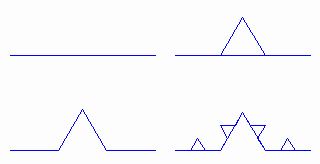
\includegraphics[width=7cm]{ressources/koch_etapes.png}
&
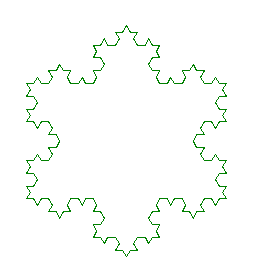
\includegraphics[width=4cm]{ressources/flocon.png}\\
Les 4 premières étapes & Flocon de von Koch
\end{tabular} 
\end{center}
\begin{center}
\shadowbox{\parbox{10cm}{\centering L'objectif de cette séance est de créer un programme récursif permettant de dessiner un flocon de von Koch}}
\end{center}
\section{Module Turtle}
La bibliothèque \emph{Turtle} permet de dessiner des figures géométriques simplement. La documentation se trouve ici:
\begin{center}
\url{https://docs.python.org/fr/3.8/library/turtle.html}
\end{center}
\begin{activite}
Découverte de la bibliothèque \emph{Turtle}.
\begin{enumerate}
\item Importer la bibliothèque \emph{turtle}.
\item Dessiner un carré de 100 de côté.
\item Dessiner la figure \ref{etoile} composée de 10 carrés.
\item Écrire une fonction \textbf{hex\_couleur() $\rightarrow$ str} qui renvoie une couleur aléatoire en écriture hexadécimal. Rappel: une couleur s'écrit sous la forme \#RRGGBB (\#23A45F) où chaque paire est l'équivalent héxadécimal d'un nombre décimal compris entre 0 et 255.
\item Utiliser la fonction précédente pour colorer chaque carré.
\end{enumerate}
\end{activite}
\begin{figure}[!h]
\centering
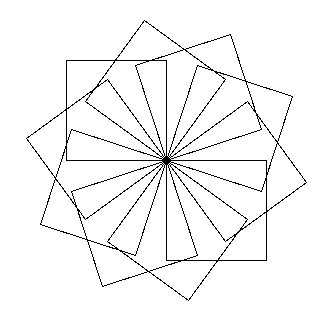
\includegraphics[width=3cm]{ressources/etoile.png}
\captionof{figure}{10 carrés}
\label{etoile}
\end{figure}
\section{Flocon de von Koch}
\subsection{Courbe de von Koch}
Avec le module \emph{Turtle} il est possible d'adapter les quatre premières étapes de la courbe de von Koch et tracer directement la figure \ref{koch1}.
\begin{figure}[!h]
\centering
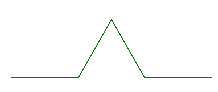
\includegraphics[width=2cm]{ressources/koch1.png}
\captionof{figure}{cas n=1}
\label{koch1}
\end{figure}
\begin{activite}
\begin{enumerate}
\item Écrire une fonction \textbf{courbe\_koch() $\rightarrow$ None} qui trace la figure \ref{koch1}.
\item Chaque segment de la figure \ref{koch1} peut être vu comme le cas où n=0. Adapter la fonction précédente en une fonction récursive \textbf{courbe\_koch(n: int,mesure: int) $\rightarrow$ None} qui dessine une courbe de von Koch de profondeur \emph{n}.
\item Tester la fonction pour plusieurs valeurs de \emph{n}  (ne pas dépasser 5).
\end{enumerate}
\end{activite}
\begin{figure}[!h]
\centering
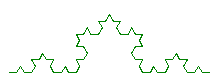
\includegraphics[width=3cm]{ressources/koch3.png}
\captionof{figure}{cas n=3}
\label{koch3}
\end{figure}
\subsection{Flocon}
\begin{activite}
Écrire une fonction \textbf{flocon(n: int,mesure: int) $\rightarrow$ None} qui utilise la fonction \emph{courbe\_koch} pour tracer le flocon entier.
\end{activite}
\begin{figure}[!h]
\centering
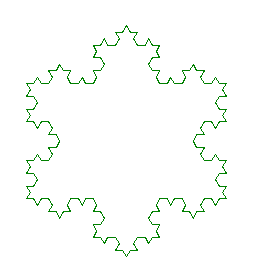
\includegraphics[width=3cm]{ressources/flocon.png}
\captionof{figure}{Flocon de von Koch}
\label{flocon}
\end{figure}
\subsection{Variantes}
\begin{activite}
Adapter le programme précédent pour utiliser la courbe de la figure \ref{kochcarre}.
\end{activite}
\begin{figure}[!h]
\centering
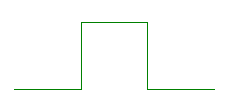
\includegraphics[width=3cm]{ressources/vonkochcarre.png}
\captionof{figure}{Variante}
\label{kochcarre}
\end{figure}
\end{Form}
\end{document}